% Clustering details removed from halfway_checkin.tex for later review.
% Each block is the original text, in report order. Not compiled on its own.

% ---------------------------------------------------------------------------
% Methods 3.4: full clustering and validation paragraph
% ---------------------------------------------------------------------------
I clustered the ten standardized style features with K-means (50 initializations) and Gaussian mixture models (GMM; full covariance, 10 initializations). I compared them with silhouette scores, and the GMMs with BIC. Since a style label isn't much use if it changes every time you refit, I ran five checks on the two-cluster solution:
\begin{enumerate}
  \item agreement between K-means and the GMM (adjusted Rand index, ARI);
  \item re-clustering on only the more reliable score mix and consistency features;
  \item a stricter threshold of 3 events, 6 rounds and 108 holes;
  \item 50 bootstrap resamples of players, refitting each and relabeling the original players;
  \item PCA, to see whether the data look like separate groups or one continuous cloud.
\end{enumerate}
Rating and strokes gained per 18 aren't clustering inputs. I only use them afterwards to check whether the clusters are just picking up skill.

% ---------------------------------------------------------------------------
% Results 4.1: choosing the number of clusters (text + Table 2, model sweep)
% ---------------------------------------------------------------------------
\subsection{Choosing the number of clusters}

Table~\ref{tab:sweep} shows the results for 2 to 8 clusters. BIC is lowest at three, but silhouette scores are low across the board (0.165 at most) and drop off for GMMs past three clusters. I started with the three-cluster GMM since it had the best BIC. Its smallest cluster was 56 players with a median rating of 821, separated mostly by high round-to-round variance. That looked like a group of lower-rated, less consistent players, not a play style. So I switched to two clusters. If the data won't split cleanly into two groups, I don't think more groups would be convincing either.

\begin{table}[H]
\centering
\footnotesize
\setlength{\tabcolsep}{8pt}
\renewcommand{\arraystretch}{0.92}
\caption{Silhouette and BIC for 2 to 8 clusters on the ten skill-adjusted features, 604 players ($k = 7$ left out; it follows the same trend). A silhouette around 0.5 or higher would mean well-separated clusters.}
\label{tab:sweep}
\begin{tabular}{@{}rrrr@{}}
\toprule
\textbf{$k$} & \textbf{K-means silhouette} & \textbf{GMM silhouette} & \textbf{GMM BIC} \\
\midrule
2 & \textbf{0.165} & \textbf{0.158} & 8,878 \\
3 & 0.122 & 0.145 & \textbf{8,754} \\
4 & 0.120 & 0.104 & 8,986 \\
5 & 0.125 & 0.033 & 9,135 \\
6 & 0.122 & $-0.010$ & 9,376 \\
8 & 0.117 & 0.015 & 9,880 \\
\bottomrule
\end{tabular}
\end{table}

% ---------------------------------------------------------------------------
% Results 4.2: opening paragraph with cluster sizes and SD values
% ---------------------------------------------------------------------------
\subsection{Two clusters: steady and volatile}

The two-cluster GMM puts 194 players in cluster 0 and 410 in cluster 1. Figure~\ref{fig:centroids} shows the cluster means. Compared with players at a similar performance level, cluster 0 makes fewer pars ($-0.7$ SD) and birdies ($-0.4$ SD), more bogeys ($+0.6$ SD) and more doubles or worse ($+0.9$ SD), and has higher hole volatility ($+0.7$ SD). Cluster 1 is the opposite, but closer to zero because it's the bigger group. Both clusters are near zero on the hole type features. So what separates them is how consistently players score, not which kinds of holes they do well on. I'll call cluster 0 ``volatile'' and cluster 1 ``steady''.

% ---------------------------------------------------------------------------
% Results 4.2: variance medians sentence
% ---------------------------------------------------------------------------
It also has higher round-to-round SD (4.49 vs.\ 4.00) and hole volatility (0.82 vs.\ 0.73).

% ---------------------------------------------------------------------------
% Results 4.3: robustness paragraph + Table 3 (stability checks) + Figure 6 (PCA)
% ---------------------------------------------------------------------------
\subsection{Robustness}

Table~\ref{tab:robust} lists the stability checks. The two-cluster split holds up reasonably well when I switch algorithms or tighten the threshold, and it separates better when I cluster on only the more reliable features (silhouette 0.238 instead of 0.158). The bootstrap is less reassuring. Mean agreement with the original clusters is 0.57, and one resample gave a split basically unrelated to the original (ARI $-0.01$). The first two principal components only explain 39.7\% of the variance (22.9\% and 16.8\%). In the PCA plot (Figure~\ref{fig:pca}) the clusters look like two halves of one cloud, split mostly along PC1, and not like two separate groups.

\suppressfloats[t]
\begin{figure}[t]
\centering
\begin{minipage}[t]{0.53\textwidth}
  \vspace{0pt}
  \centering
  \footnotesize
  \setlength{\tabcolsep}{4pt}
  \renewcommand{\arraystretch}{0.92}
  \captionof{table}{Stability checks for the two-cluster solution.}
  \label{tab:robust}
  \begin{tabularx}{\linewidth}{@{}YY@{}}
  \toprule
  \textbf{Check} & \textbf{Result} \\
  \midrule
  K-means vs.\ GMM (same features) & ARI 0.585 \\
  Reliable features only (6 score mix and consistency features) & GMM silhouette 0.238 (vs.\ 0.158); ARI 0.625 with all-feature GMM \\
  Stricter threshold: 3 events, 6 rounds, 108 holes (432 players) & ARI 0.893 on common players \\
  Bootstrap, 50 resamples & mean ARI 0.572, median 0.623, min $-0.012$ \\
  PCA, first two components & 39.7\% of variance \\
  \bottomrule
  \end{tabularx}
\end{minipage}\hfill
\begin{minipage}[t]{0.43\textwidth}
  \vspace{0pt}
  \centering
  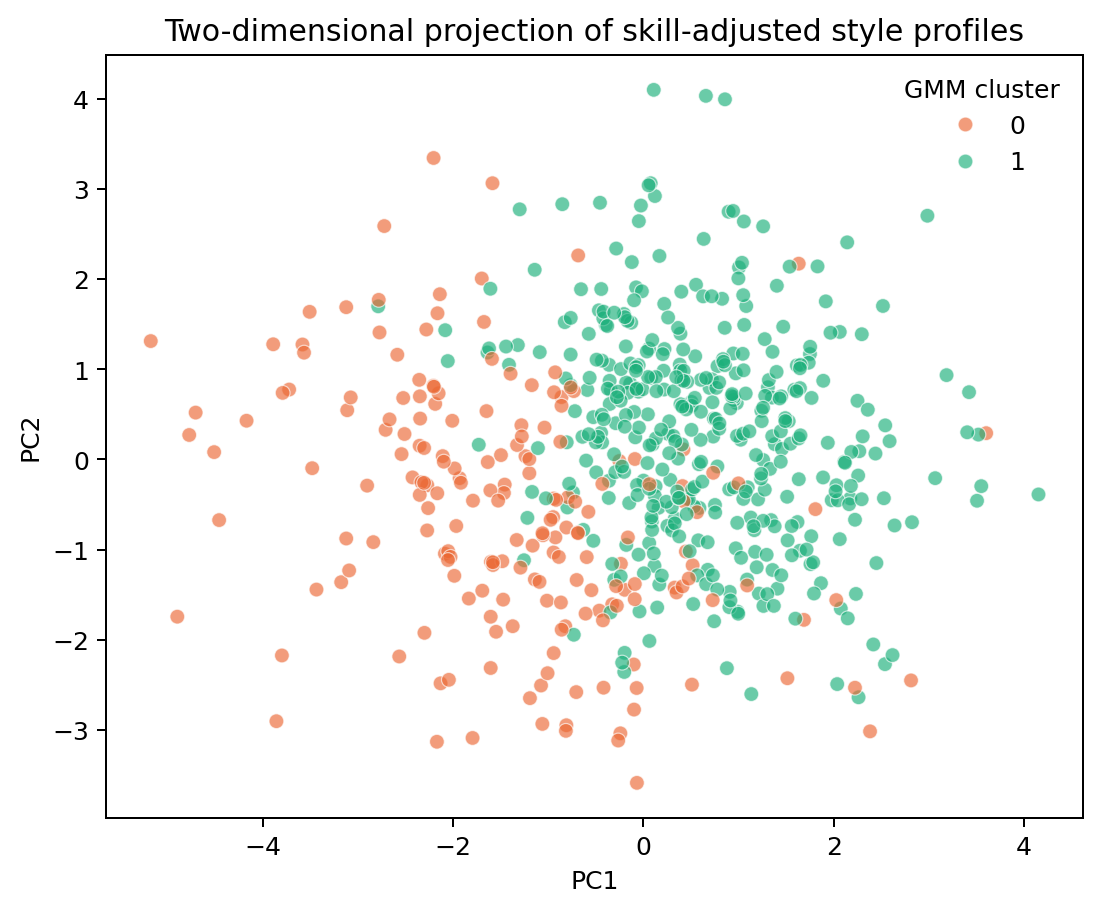
\includegraphics[width=\linewidth]{figures/clustering_pca.png}
  \caption{Skill-adjusted profiles on the first two principal components (39.7\% of variance), colored by GMM cluster.}
  \label{fig:pca}
\end{minipage}
\end{figure}

% ---------------------------------------------------------------------------
% Limitations: sample size bullet
% ---------------------------------------------------------------------------
(ARI 0.89) after 'The stricter threshold gives similar clusters'

